\documentclass[12pt, a4paper]{article}
\usepackage{amsmath}
\usepackage{amsfonts}
\usepackage{amsthm}
\usepackage{mathtools}
\newtheorem{theorem}{Theorem}
\usepackage{pgfplots}
\pgfplotsset{width=10cm,compat=1.9}

\begin{document}

\section{Bayesian statistics}

\textit{Bayesian statistics}, as opposed to frequentist statistics, views probabilities merely as current opinion regarding the true state of the world. As new data is brought to light such opinion will be revised to reflect the new evidence. The way to update probabilities is prescribed by Bayes' theorem.\par
So Bayesian probabilities are subjective, in contrast to the objective probabilities of frequentist statistics.

\subsection{Prior and posterior probablities}
Assume we have a given probability of an event $A$ happening. This probability $P(A)$ is known as the \textit{prior} in Bayesian terminology. Now, assume we know that event $B$ has occured - this constitutes evidence. We should now adjust our probability of event $A$ to the conditional probability $P(A|B)$, which is known as the \textit{posterior}. The two are related by Bayes' theorem:
\begin{equation}
\label{bayes}
P(A|B)=\frac{P(B|A)P(A)}{P(B)}
\end{equation}

\subsection{Example: Radio quality}
A given corporation produces radios. Of the last 200 truckloads of radios, 128 have been "bad" and 72 "good"; In the bad truckloads 44\% of the radios were defective. In the good truckloads only 15\%. Now, we're faced with determining whether a new truckload of radios is good or bad. Initially, since all we have is the information that 128 out of 200 truckloads have been bad, our prior probabilities would be:
\begin{equation}
P(B)=\frac{128}{200}=64\%,\quad P(G)=\frac{72}{200}=36\%
\end{equation}
Here, $B$ refers to the event "Bad truckload", and $G$ to the event "Good truckload". However, we now sample one of the radios from the truckload. This radio turns out to be defective. What are the updated, posterior probabilities of the truckload being good or bad? To answer this, we need Bayes' theorem:
\begin{equation}
\label{radio_post}
P(B|D)=\frac{P(D|B)P(B)}{P(D)}
\end{equation}
Here $D$ refers to the event "Defective radio". $P(D|B)$ is the probability of a radio in a bad truckload being defective. We know that this is 44\%. We know that $P(B)=64\%$. But what is $P(D)$? By the law of total probability, this is:
\begin{equation}
P(D)=P(D|B)P(B)+P(D|G)P(G)=44\%\cdot 64\% + 15\%\cdot 36\% = 33.56\%
\end{equation}
Now, we can insert into equation $(\ref{radio_post})$:
\begin{equation}
P(B|D)=\frac{44\%\cdot 64\%}{33.56\%}=83.9\%
\end{equation}
By symmetry, the posterior probability of a good truckload has shrunk to $P(G|D)=100\%-83.9\%=16.1\%$. The knowledge that the sample radio is defect makes us update our view of the world.

\subsubsection{Radio quality with odds}
One could also reformulate the example above using \textit{odds}. The odds of a bad truckload is:
\begin{equation}
\frac{P(B)}{P(G)}=\frac{64\%}{36\%}=1.78
\end{equation} 
These are the prior odds. After the reveal of the defect radio, odds are:
\begin{equation}
\frac{P(B|D)}{P(G|D)}=\frac{83.9\%}{16.1\%}=5.21
\end{equation}
These are the posterior odds. How are the two related? Let's use Bayes' theorem to find out:
\begin{equation}
\frac{P(B|D)}{P(G|D)}=\frac{P(D|B)P(B)/P(D)}{P(D|G)P(G)/P(D)}=\frac{P(D|B)P(B)}{P(D|G)P(G)}
\end{equation}
So the prior odds times the quantity $\frac{P(D|B)}{P(G|B)}$, which can be interpreted as a \textit{likelihood ratio}. The relation between these three quantities can be written:
\begin{equation}
\label{bayes_odds}
\textrm{posterior odds}=\textrm{likelihood ratio}\cdot\textrm{prior odds}
\end{equation}

\subsection{Calculating posterior probabilities}
In general, let $\theta$ be a parameter (or a vector of parameters) used to describe an event. In the example above, $\theta$ covered two option: Good or Bad truckload. In general, $\theta$ may represent many - even infinitely many - different outcomes. Let $X$ represent new evidence. By Bayes' theorem:
\begin{equation}
P(\theta|X)=\frac{P(X|\theta)P(\theta)}{P(X)}
\end{equation}
For a given set of evidence $X$ we wish to update on, $P(X)$ is a constant, so this may also be expressed:
\begin{equation}
\label{bayes_prob}
P(\theta|X)\propto P(X|\theta)P(\theta)
\end{equation}
Or reworded to resemble equation $(\ref{bayes_odds})$:
\begin{equation}
\label{bayes_prob2}
\textrm{posterior probability}\propto\textrm{likelihood}\cdot\textrm{prior probability}
\end{equation}

\subsubsection{Radio quality revisited}
The radio manufacturing company from above have made further inquiries into the distribution of percentages of defective radios in a truckload. In this situation, the general parameter $\theta$ from last section corresponds to the defective percentage, which we will call $\pi$. It turns out, that this percentage seems to follow a beta distribution with parameters $\alpha=2$ and $\beta=4$:
\begin{equation}
P(\pi)\propto\pi(1-\pi)^3
\end{equation}
Since beta distributions are continuous, this is a probability \textit{density} of finding a truckload with a defective percentage of $\pi$, rather than a probability - this is our prior. We're now presented with a new truckload of radios. Without any further information, our best bet is the prior distribution. However, we now inspect the truckload, taking a random sample of 5 radios. It turns out, that 3 of those are defective. How do we account for this new information to update our distribution? According to equation $(\ref{bayes_prob})$, we need to find the likelihood $P(X|\pi)$. Here $X$ refers to the evidence of getting 3 out of 5 defective radios. In other words, this is a binomial likelihood\footnote{This assumes that the truckload is large enough that the consecutive picking of radios to test does not affect $\pi$ significantly.}:
\begin{equation}
P(X|\pi)=\binom{5}{3}\pi^3(1-\pi)^2\propto\pi^3(1-\pi)^2
\end{equation}
So the posterior distribution also turns out to be a beta distribution:
\begin{equation}
P(\pi|X)\propto\pi^4(1-\pi)^5
\end{equation}
This is a beta distribution with parameters $\alpha=5$ and $\beta=6$. When both distributions are of the same type, we speak of \textit{conjugate distributions}. Given a likelihood function, a prior that makes the distributions conjugate is known as a \textit{conjugate prior}.\par
The graph below shows the three distributions for comparison\footnote{The likelihood isn't a distribution, since it does not sum to 1. However, for clarity, in this figure it has been scaled as if it did.}. The prior is relatively optimistic regarding quality, and the likelihood less so. The posterior is a compromise between the two.

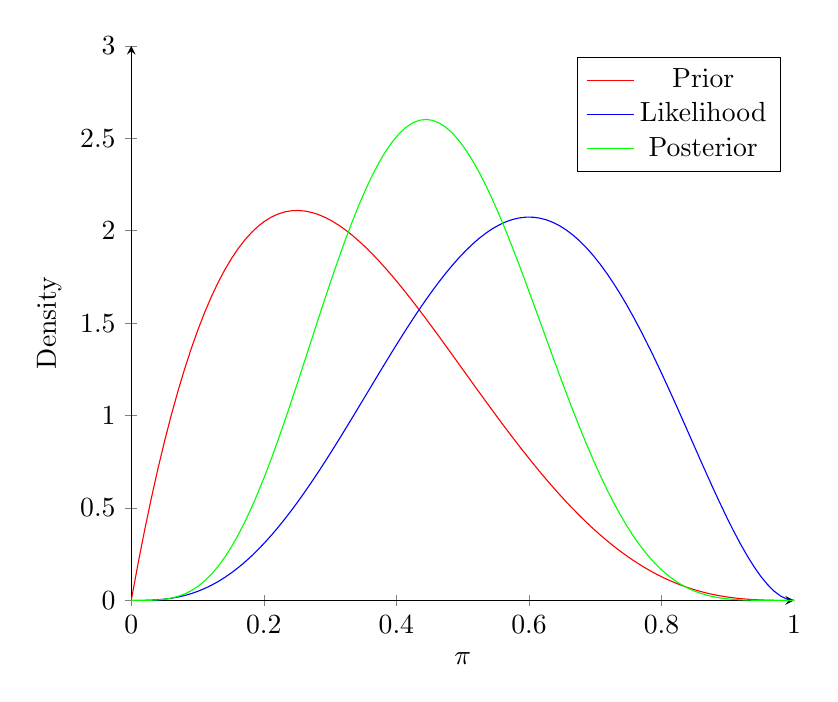
\begin{tikzpicture}
\begin{axis}[
    axis lines = left,
    xlabel = $\pi$,
    ylabel = Density,
    ymin = 0,
    ymax = 3,
]
\addplot [
    domain=0:1, 
    samples=100, 
    color=red,
]
{20 * x * (1-x)^3};
\addlegendentry{Prior}
\addplot [
    domain=0:1, 
    samples=100, 
    color=blue,
    ]
    {60 * x^3 * (1-x)^2};
\addlegendentry{Likelihood}
\addplot [
    domain=0:1, 
    samples=100, 
    color=green,
    ]
    {1260 * x^4 * (1-x)^5};
\addlegendentry{Posterior}
 
\end{axis}
\end{tikzpicture}

\end{document}


